\documentclass[handout,11pt,aspectratio=169]{beamer}

\usetheme{Singapore}
\usecolortheme{orchid}

\usepackage[utf8]{inputenc}
\usepackage[russian]{babel}
\usepackage{amsmath}
\usepackage{amsfonts}
\usepackage{amssymb}
\usepackage{graphicx}
\usepackage{bibentry}
\usepackage{wasysym}
\usepackage[most]{tcolorbox}
\usepackage[normalem]{ulem}

\usepackage{hyperref}

\definecolor{info}{RGB}{62, 180, 137}
\definecolor{warn}{RGB}{128, 0, 0}

\author{Николай Анохин}
\title{Recommendations + Reinforcement Learning = \ensuremath\heartsuit}

\logo{
\includegraphics[width=.05\textwidth]{images/ok_logo.png}}

\AtBeginSection[]{
  \begin{frame}
  \vfill
  \centering
  \begin{beamercolorbox}[sep=8pt,center,shadow=true,rounded=true]{title}
    \usebeamerfont{title}\insertsectionhead\par
  \end{beamercolorbox}
  \vfill
  \end{frame}
}

\begin{document}

{
\setbeamertemplate{headline}{}

\begin{frame}
\titlepage
\end{frame}

%\begin{frame}
%\tableofcontents
%\end{frame}

}

\begin{frame}{Контекст}

\begin{center}
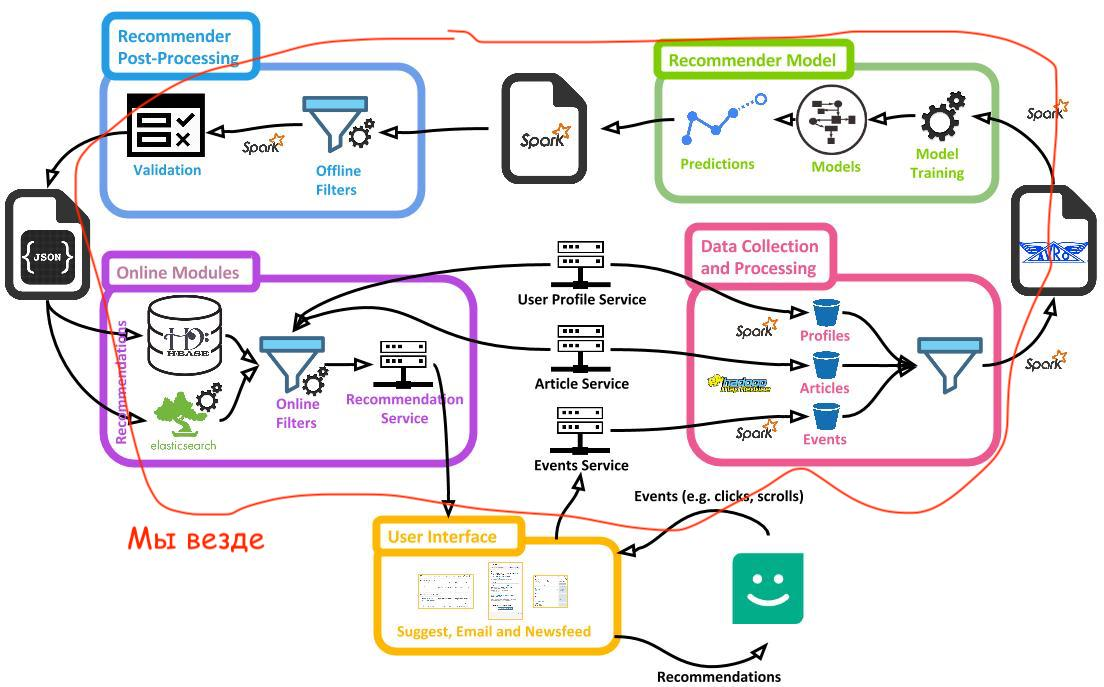
\includegraphics[scale=0.23]{images/mendeley.jpeg}
\end{center}

\end{frame}

\begin{frame}{Сложности в постановке задачи рекомендаций}

\begin{enumerate}
\item Оцениваем айтемы по-отдельности, а показываем по несколько (лентой)
\item Модель не объясняет, почему именно эти айтемы подходят пользователю
\item Смещение между распределениями на обучении и применении
\item {\color{blue} Не учитывается долгострочный эффект рекомендаций}
\end{enumerate}
\end{frame}

\section{Долгосрочный эффект рекомендаций}

\begin{frame}{}

\begin{center}
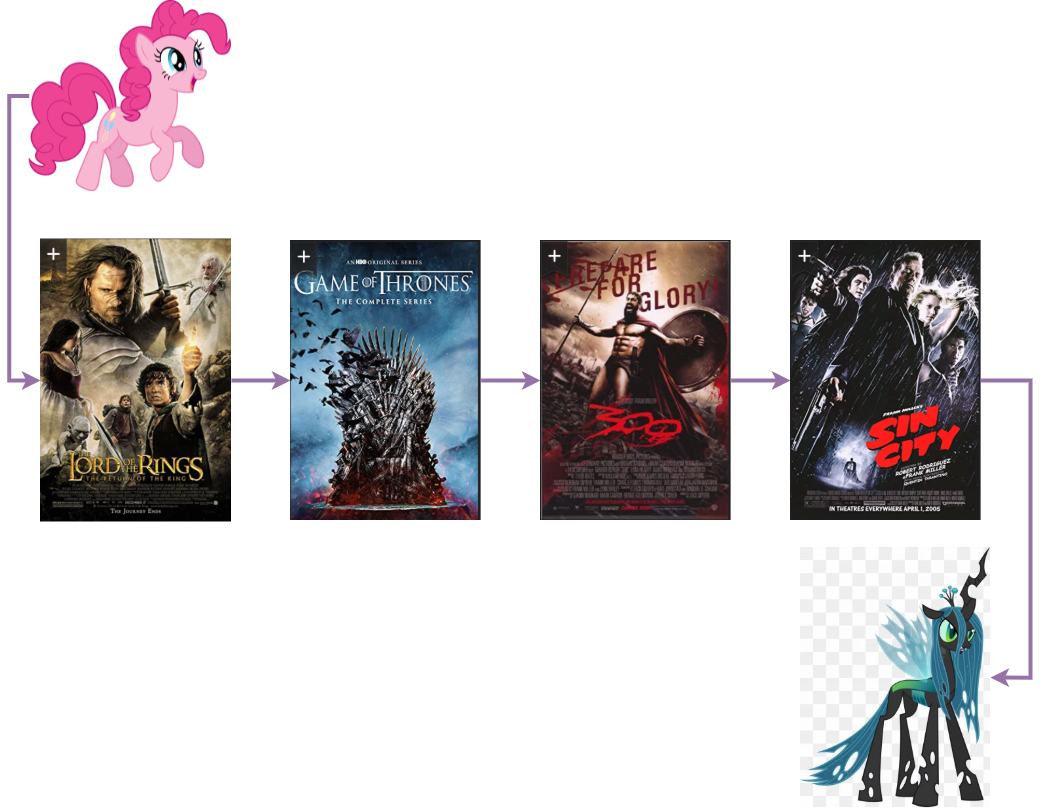
\includegraphics[scale=0.22]{images/longterm.png}
\end{center}

\end{frame}

\begin{frame}{Долгосрочный эффект рекомендаций}

\begin{tcolorbox}[colback=info!5,colframe=info!80,title=]
\begin{enumerate}[<+->]
\item Эволюция пользователя (рекомендер влияет на пользователя)
\item Эволюция рекомендера (рекомендер влияет на себя)
\item Отложенная награда
\end{enumerate}
\end{tcolorbox}

\end{frame}

\begin{frame}{Постановка задачи Reinforcement Learning}

\begin{columns}

\begin{column}{0.45\textwidth}
\begin{center}
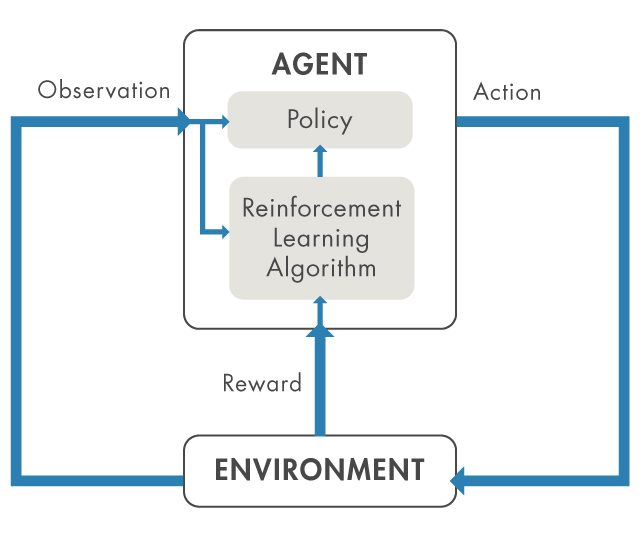
\includegraphics[scale=0.2]{images/rl.jpeg}
\end{center}
\end{column}

\begin{column}{0.45\textwidth}

\begin{small}
\begin{center}
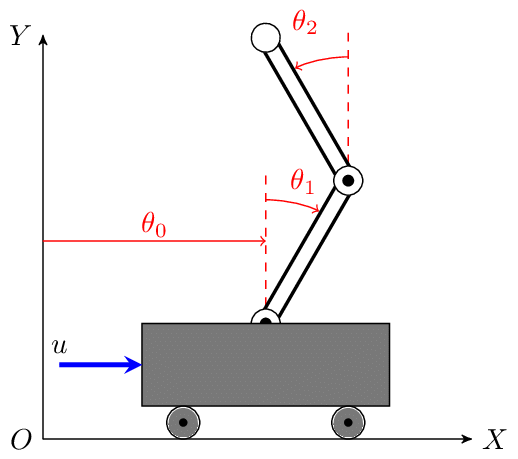
\includegraphics[scale=0.3]{images/catpole.png}
\end{center}
\end{small}

\end{column}
\end{columns}

\end{frame}

\begin{frame}{Markov Decision Process (MDP)}

\begin{small}

\begin{tabular}{l l}
История & $H_t = O_1, A_1, R_1, \ldots O_t, A_t, R_t$ \\
\pause Состояние & $S_t = f(H_t)$ \\
\pause Среда & $\mathcal{P}(S_t | A_{t}, S_{t-1})$ \\
\pause Награда & $R(S_t | S_{t-1})$ \\
\pause Политика & $\pi(A | S)$ \\
\pause Кумулятивная награда & $G_t = R_t + \gamma R_{t+1} + \gamma^2 R_{t+2} + \ldots$
\end{tabular}

\end{small}

\vfill

\pause
\begin{tcolorbox}[colback=info!5,colframe=info!80,title=Цель: выбрать оптимальную политику]
MDP: $(S,A,\mathcal{P},R)$
\[
\pi^* = \arg \max_{\pi} \mathbb{E}_{\mathcal{P}, \pi} G_t
\]
\end{tcolorbox}

\end{frame}

\begin{frame}{Рекомендации как Reinforcement Learning}

\begin{columns}

\begin{column}{0.3\textwidth}
\begin{center}
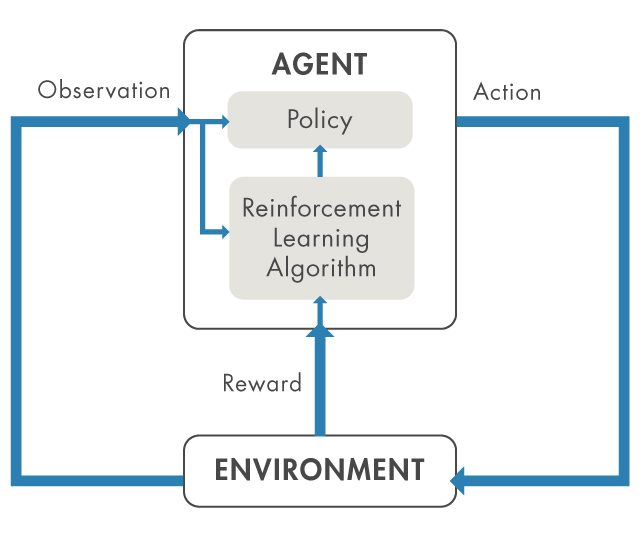
\includegraphics[scale=0.2]{images/rl.jpeg}
\end{center}
\end{column}

\begin{column}{0.65\textwidth}

\begin{footnotesize}
\begin{center}
\begin{tabular}{l c l}
RecSys & $\rightarrow$ & RL \\
\hline
Пользователь & $\rightarrow$ & \pause Среда (environment) \\
Контекст & $\rightarrow$ & \pause Наблюдение (observation) \\
Рекомендательный сервис & $\rightarrow$ &  \pause Агент (agent) \\
Алгоритм рекомендаций & $\rightarrow$ &  \pause Политика (policy) \\
Рекомендация & $\rightarrow$ & \pause Действие (action) \\ 
Покупка, просмотр, клик & $\rightarrow$ &  \pause Награда (reward) \\
??? & $\rightarrow$ &  \pause Эпизод (episode) \\
\end{tabular}
\end{center}
\end{footnotesize}

\end{column}
\end{columns}

\end{frame}

\begin{frame}{Почему RL (почти) не используется в продакшен рекомендерах?}

\begin{tcolorbox}[colback=warn!5,colframe=warn!80,title=]
\begin{itemize}[<+->]
\item Огромное меняющееся пространство действий-состояний
\item Отсутствие данных (сред) для проверки идей
\item Дорогая реализация алгоритмов
\end{itemize}
\end{tcolorbox}

\end{frame}

\section{Многорукие бандиты}

\begin{frame}{Multi-armed bandit}

\begin{center}
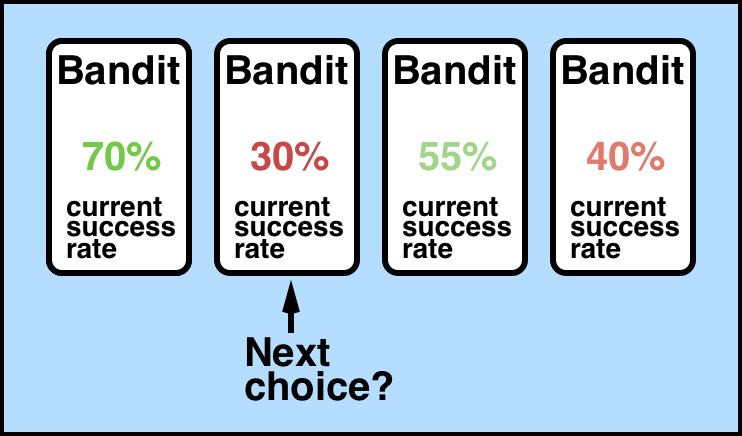
\includegraphics[scale=0.3]{images/mab.png}
\end{center}

\[
Q_n(a) = \rm I\!E[R_n \mid A_n = a]
\]
\[
A^*_n = \max_a Q_n(a)
\]

\end{frame}

\begin{frame}{Варианты решений I \cite{BANDITS1}}

\begin{itemize}
\item $\varepsilon$-greedy: выбираем случайную руку с вероятностью $\varepsilon$, иначе жадно
\item $\varepsilon$-decay: как $\varepsilon$-greedy, но уменьшаем $\varepsilon$ со временем
\[
\varepsilon(n) = \frac{1}{1 + n \beta}
\]
\item Upper Confidence Bound (UCB)
\[
A_n = \arg \max_a \left( Q_n(a) + c \sqrt{\frac{\log(n)}{N_n(a)}} \right)
\]
\end{itemize}

\end{frame}

\begin{frame}{Варианты решений II: Gradient Bandit \cite{BANDITS2}}

Политика, которая чаще выбирает "хорошие" руки

$H(A_k)$ -- value руки $k$
\[
\pi(A_k) = \frac{\exp H(A_k)}{\sum_j \exp H(A_j)}
\]
Обновление
\[
H_{t+1} (A_t) = H_t(A_t) + \alpha (R_t - \bar R_t)(1 - \pi_t(A_t))
\]
\[
H_{t+1} (a) = H_t(a) - \alpha (R_t - \bar R_t)\pi_t(a), \; \forall a \neq A_t
\]

\end{frame}

\begin{frame}{Варианты решений III: Thompson Sampling}

\begin{columns}

\begin{column}{0.4\textwidth}
\begin{enumerate}
\item Для каждой руки оцениваем распределение награды
\item Семплируем значение из каждого из распределений
\item Выбираем руку с наибольшим значением
\end{enumerate}
\end{column}

\begin{column}{0.55\textwidth}

\begin{small}
\begin{center}
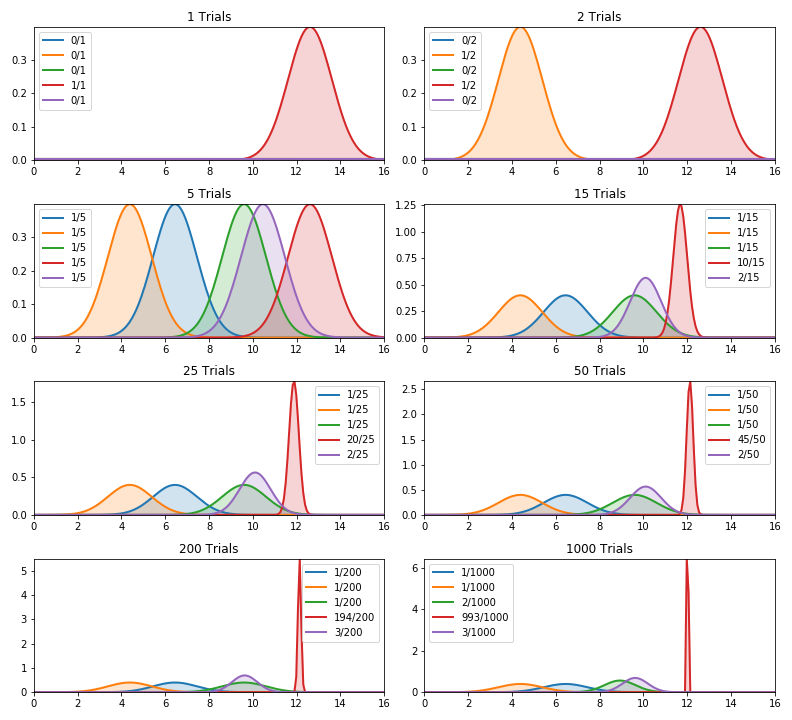
\includegraphics[scale=0.2]{images/thompson.png}
\end{center}
\end{small}

\end{column}
\end{columns}

\end{frame}

\begin{frame}{Сравнение алгоритмов \cite{BANDITS3}}

\begin{center}
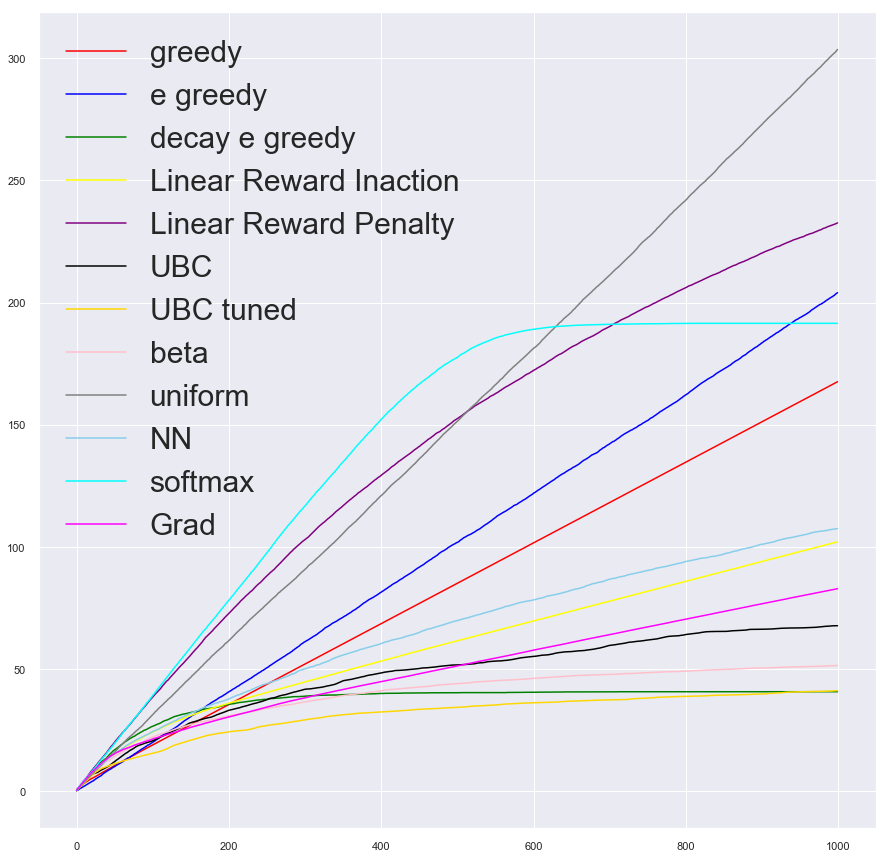
\includegraphics[scale=0.2]{images/regret.png}
\end{center}
\[
Regret_t = G_t^{optimal} - G_t
\]

\end{frame}

\begin{frame}{Итоги}

\begin{tcolorbox}[colback=info!5,colframe=info!80,title=]
\begin{itemize}
\item (В некоторых случаях) оптимально соблюдают баланс Explore/Exploit
\item Простые и работают на практике для задач с небольшим количеством действий
\end{itemize}
\end{tcolorbox}

\vfill

\begin{tcolorbox}[colback=warn!5,colframe=warn!80,title=]
\begin{itemize}
\item Не учитывают состояния среды
\end{itemize}
\end{tcolorbox}

\end{frame}

\section{Симуляторы для рекомендаций}

\begin{frame}{RecSim: A Configurable Simulation Platform for Recommender Systems \cite{RECSIM}}

\begin{center}
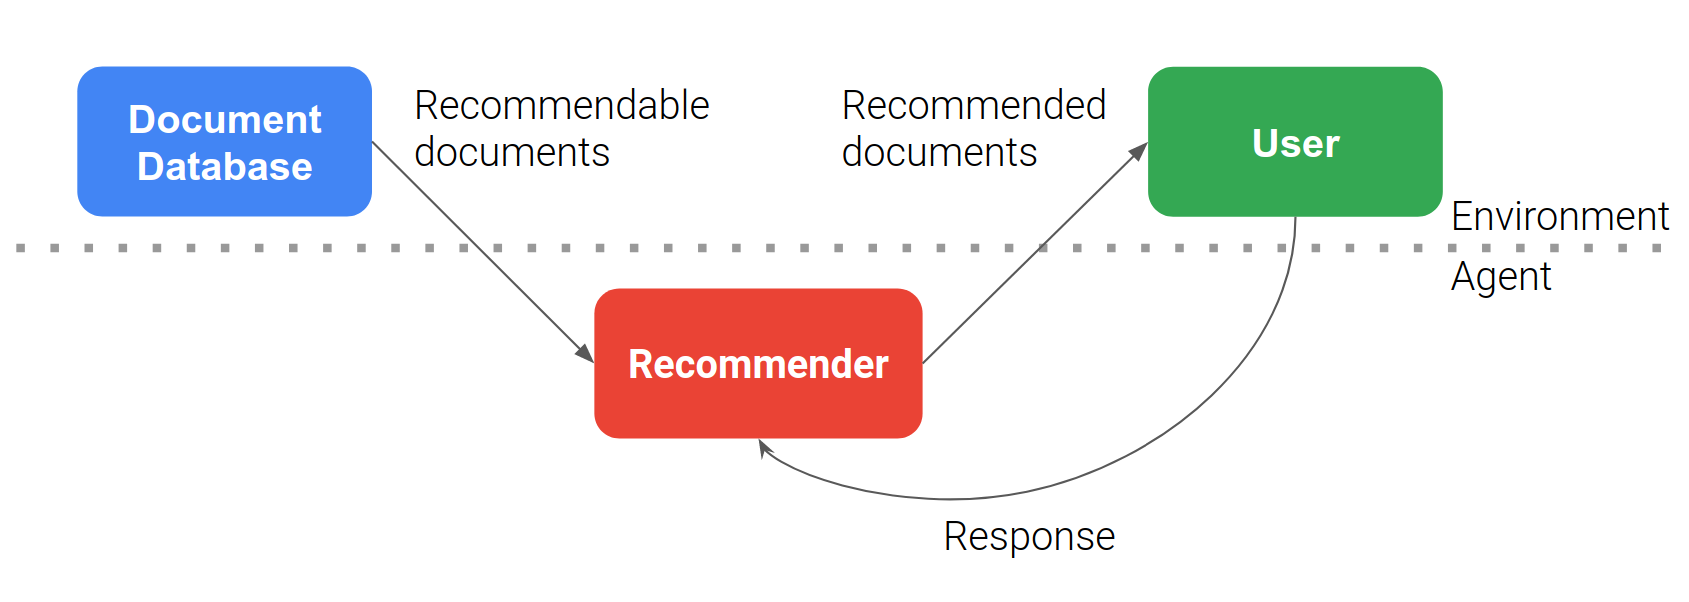
\includegraphics[scale=0.2]{images/recsim.png}
\end{center}

\end{frame}

\section{Полная постановка RL в рекомендациях}

\begin{frame}{Deep Reinforcement Learning in Large Discrete Action Spaces \cite{DDPG}\footnote{Пример использования в рекомендациях: \url{https://arxiv.org/abs/1811.05869}}}

\begin{columns}
\begin{column}{0.4\textwidth}
\begin{center}
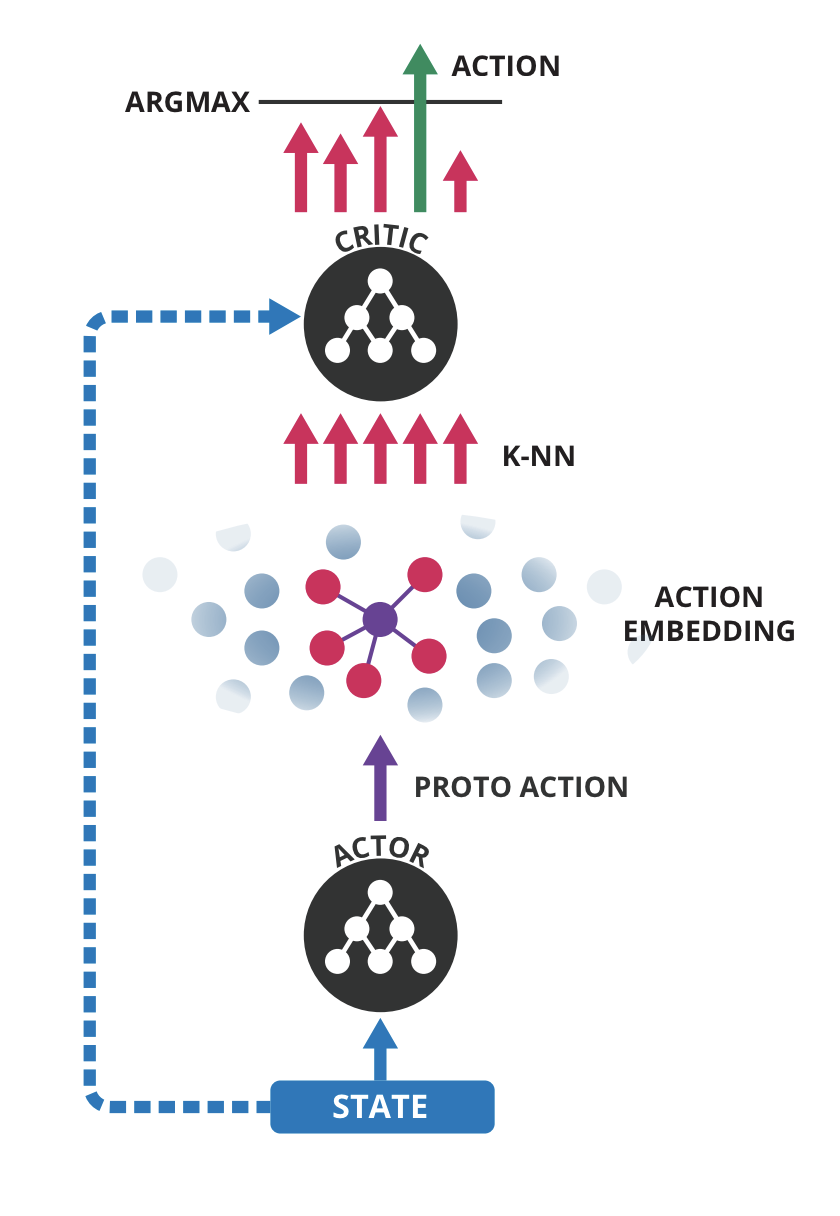
\includegraphics[scale=0.25]{images/ddpg.png}
\end{center}
\end{column}

\begin{column}{0.5\textwidth}
\begin{center}
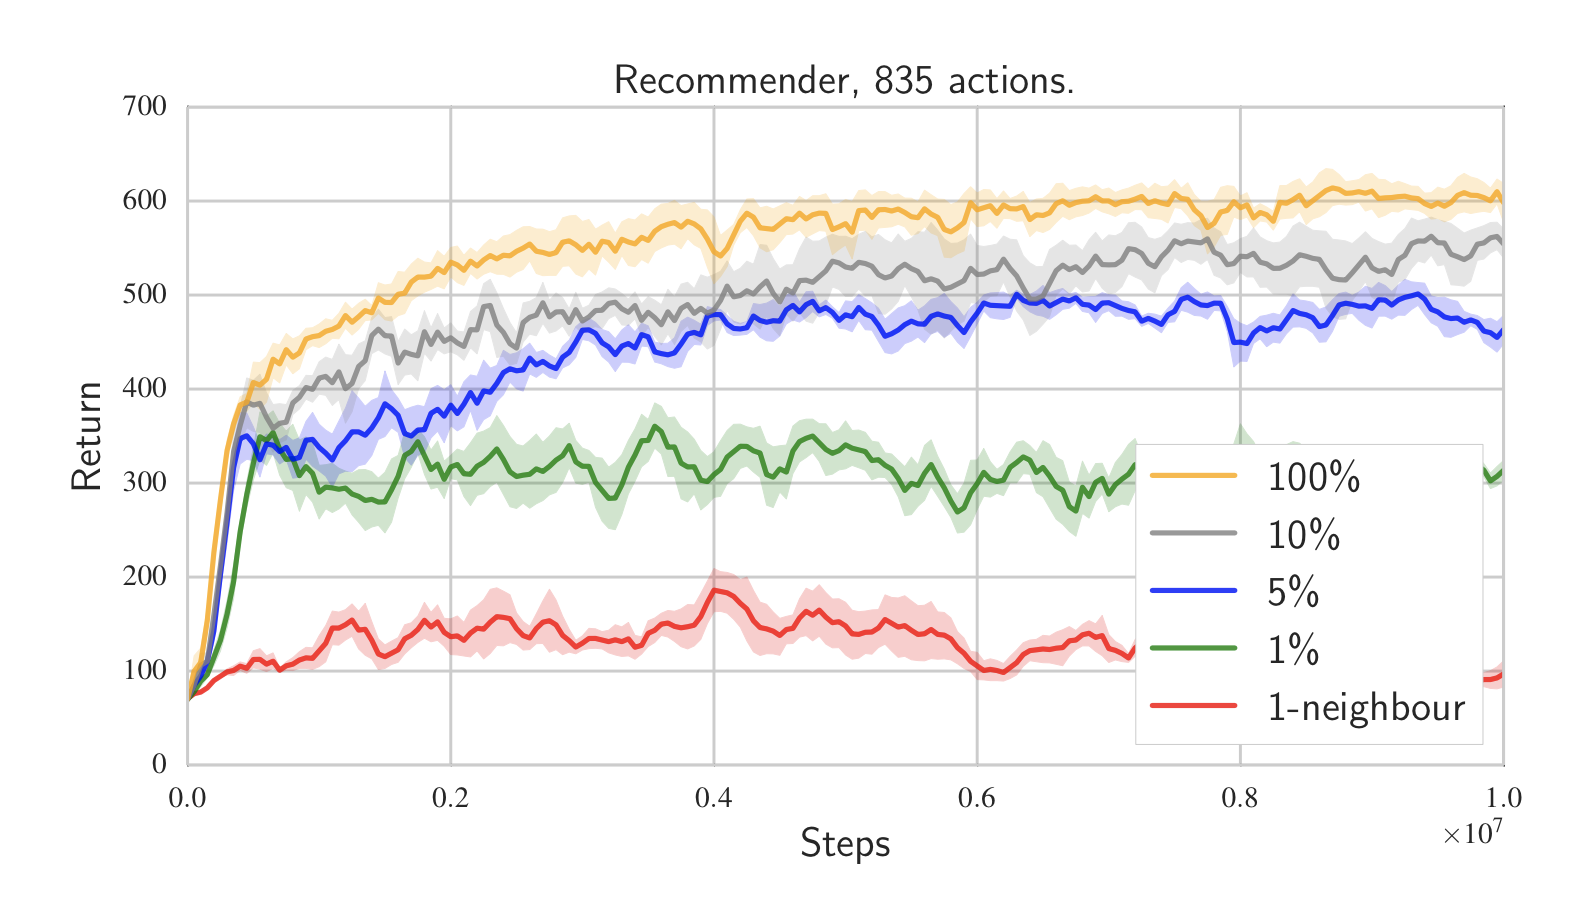
\includegraphics[scale=0.25]{images/ddpg-result.png}
\end{center}
\end{column}
\end{columns}

\end{frame}

\begin{frame}{Top-K Off-Policy Correction for a REINFORCE Recommender System
 \cite{TOPK}}
 
\begin{itemize}
\item Масштабировали алгоритм REINFORCE на огромное пространство действий.
\item Применили корректировкуу смещения между logging и обучаемой политикой.
\item Изобрели новую корректировку на top-k рекомендации.
\item Применили все это в продакшене YouTube.
\end{itemize}

\begin{center}
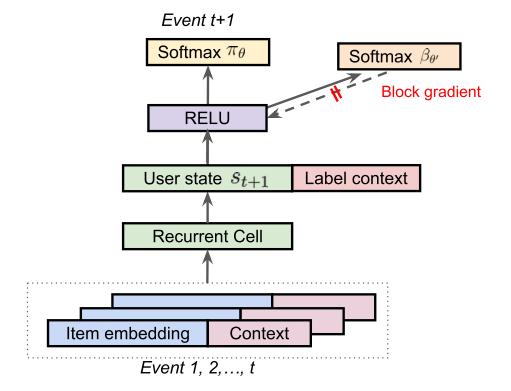
\includegraphics[scale=0.25]{images/topk.png}
\end{center}

\end{frame}

\section{Итоги}

\begin{frame}{Итоги}

\begin{tcolorbox}[colback=info!5,colframe=info!80,title=]
Постановка задачи RL очень хорошо соответствует задаче рекомендаций.
\end{tcolorbox}

\vfill

\begin{tcolorbox}[colback=info!5,colframe=info!80,title=]
В рекомендациях все признают проблемы explore/exploit и смещений. Их решают методами, заимствованными из RL.
\end{tcolorbox}

\vfill

\begin{tcolorbox}[colback=warn!5,colframe=warn!80,title=]
Придется подождать, пока RL в рекомендациях станет общей практикой.
\end{tcolorbox}

\end{frame}

\begin{frame}{Итоги курса}

\begin{tcolorbox}[colback=info!5,colframe=info!80,title=]
В будущем рекомендательные системы будут давать релевантные, разнообразные и полезные рекомендации. Они будут учитывать долгосрочные интересы пользователей. А пользователи будут понимать, почему им что-то предлагают и смогут котролировать механизмы построения рекомендаций.
\end{tcolorbox}

\begin{tcolorbox}[colback=info!5,colframe=info!80,title=]
Но понадобится ваша помощь. И научная честность.
\end{tcolorbox}

\end{frame}

\begin{frame}

\begin{center}
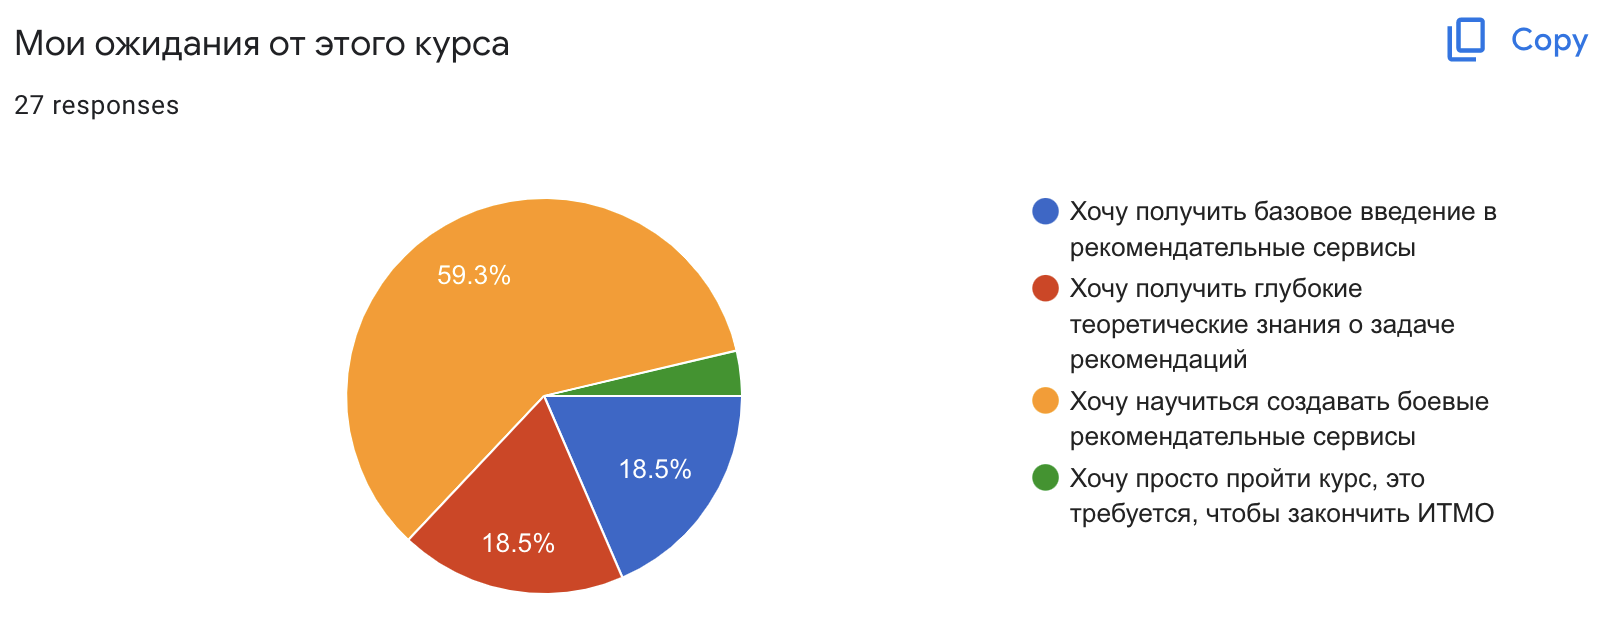
\includegraphics[scale=0.5]{images/poll.png}
\end{center}

\end{frame}

\begin{frame}

\begin{center}

\includegraphics[scale=0.4]{images/thankyou.jpeg}

\end{center}

\end{frame}

\begin{frame}[allowframebreaks]{Литература}

\bibliographystyle{amsalpha}
\bibliography{references.bib}

\end{frame}

\end{document}
